\chapter{Instrukcja obsługi}
\thispagestyle{chapterBeginStyle}
\label{rozdzial4}

W tym rozdziale omówiono wymagania wobec środowiska, w którym będzie instalowana będzie opisana w pracy aplikacja. Przedstawiono procedurę instalacji oraz jak przeprowadzić podstawową konfigurację. W następnej sekcji przedstawiono kilka przykładów użycia aplikacji.

\section{Instalacja i konfiguracja}
\subsection{Wymagania sprzętowe}
Aplikacja została stworzona pod system Android Pie. Do działania jest wymagany moduł Bluetooth w wersji co najmniej 4.0 oraz posiadanie smartbanda MiBand 3. Do zainstalowania aplikacji potrzeba minimalnie około 23 MB wolnego miejsca. 
\subsection{Instalacja}
Aplikację można zainstalować przy użyciu dołączonego do pracy pliku \textit{lockband.apk}. Aby umożliwić instalowanie aplikacji z plików APK należy nadać odpowiedniej aplikacji (w tym przypadku menadżerowi plików) pozwolenie na instalowanie nieznanych aplikacji. Lokalizacja tego ustawienia może się znacząco różnić w zależności od wersji nakładki systemowej. Następnie należy pobrać plik APK na smartfona. W kolejnym kroku należy znaleźć pobrany wcześniej plik korzystając z menedżera plików. Ostatnim krokiem jest stuknięcie w plik APK, by uruchomić instalację.
\subsection{Pierwsze uruchomienie}
Podczas pierwszego uruchomienia aplikacja na początku prosi o udzielenie potrzebnych pozwoleń: Lokalizacji, potrzebnej do korzystania z Bluetooth oraz Dostępu do danych o użyciu, koniecznych do monitorowania wyświetlanych aplikacji. Użytkownik zostaje przekierowany do ustawień, gdzie może udzielić pozwolenia na wykorzystanie danych o użyciu. Następnie użytkownik może powrócić do aplikacji, gdzie zostanie wyświetlony monit o udzielenie pozwolenia na dostęp do lokalizacji. 
\begin{figure}[H]
    \begin{center}
        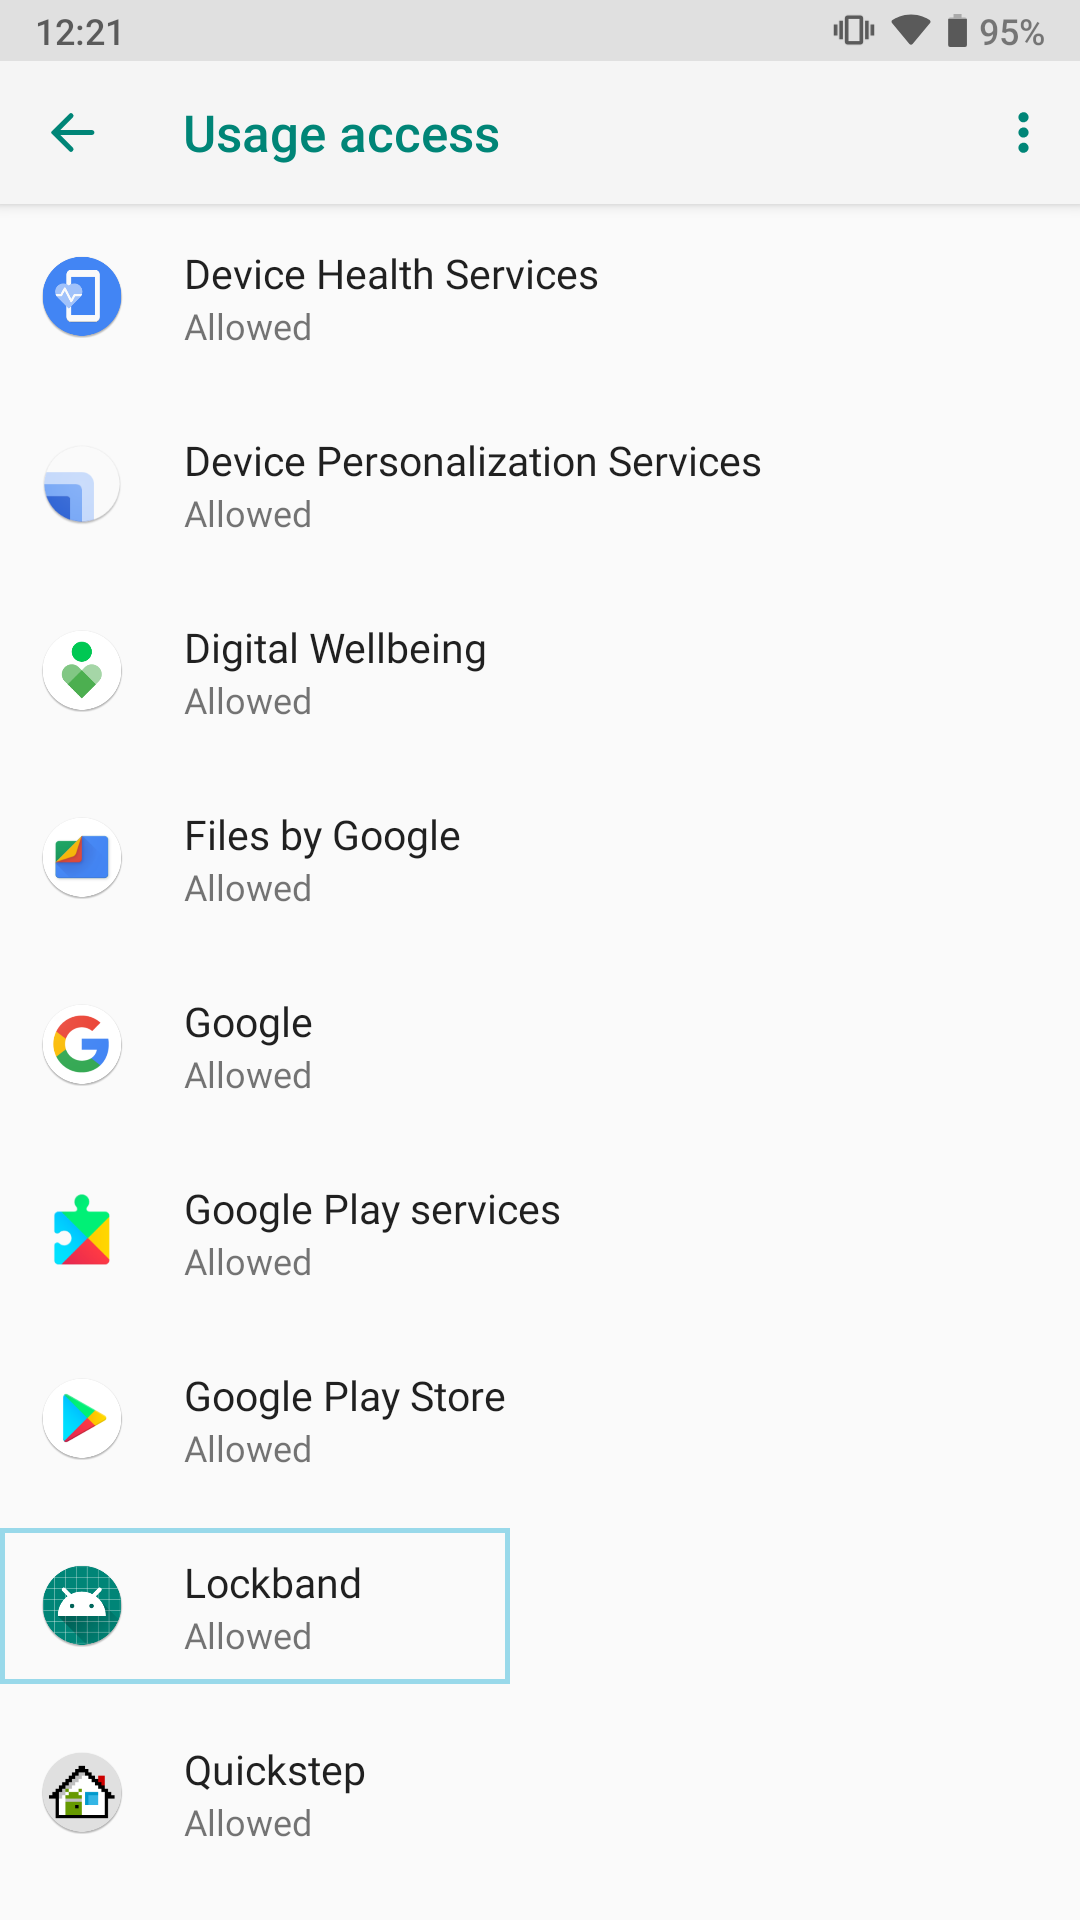
\includegraphics[width=0.27\textwidth]{app_screenshots/usage_stats_permission.png}
        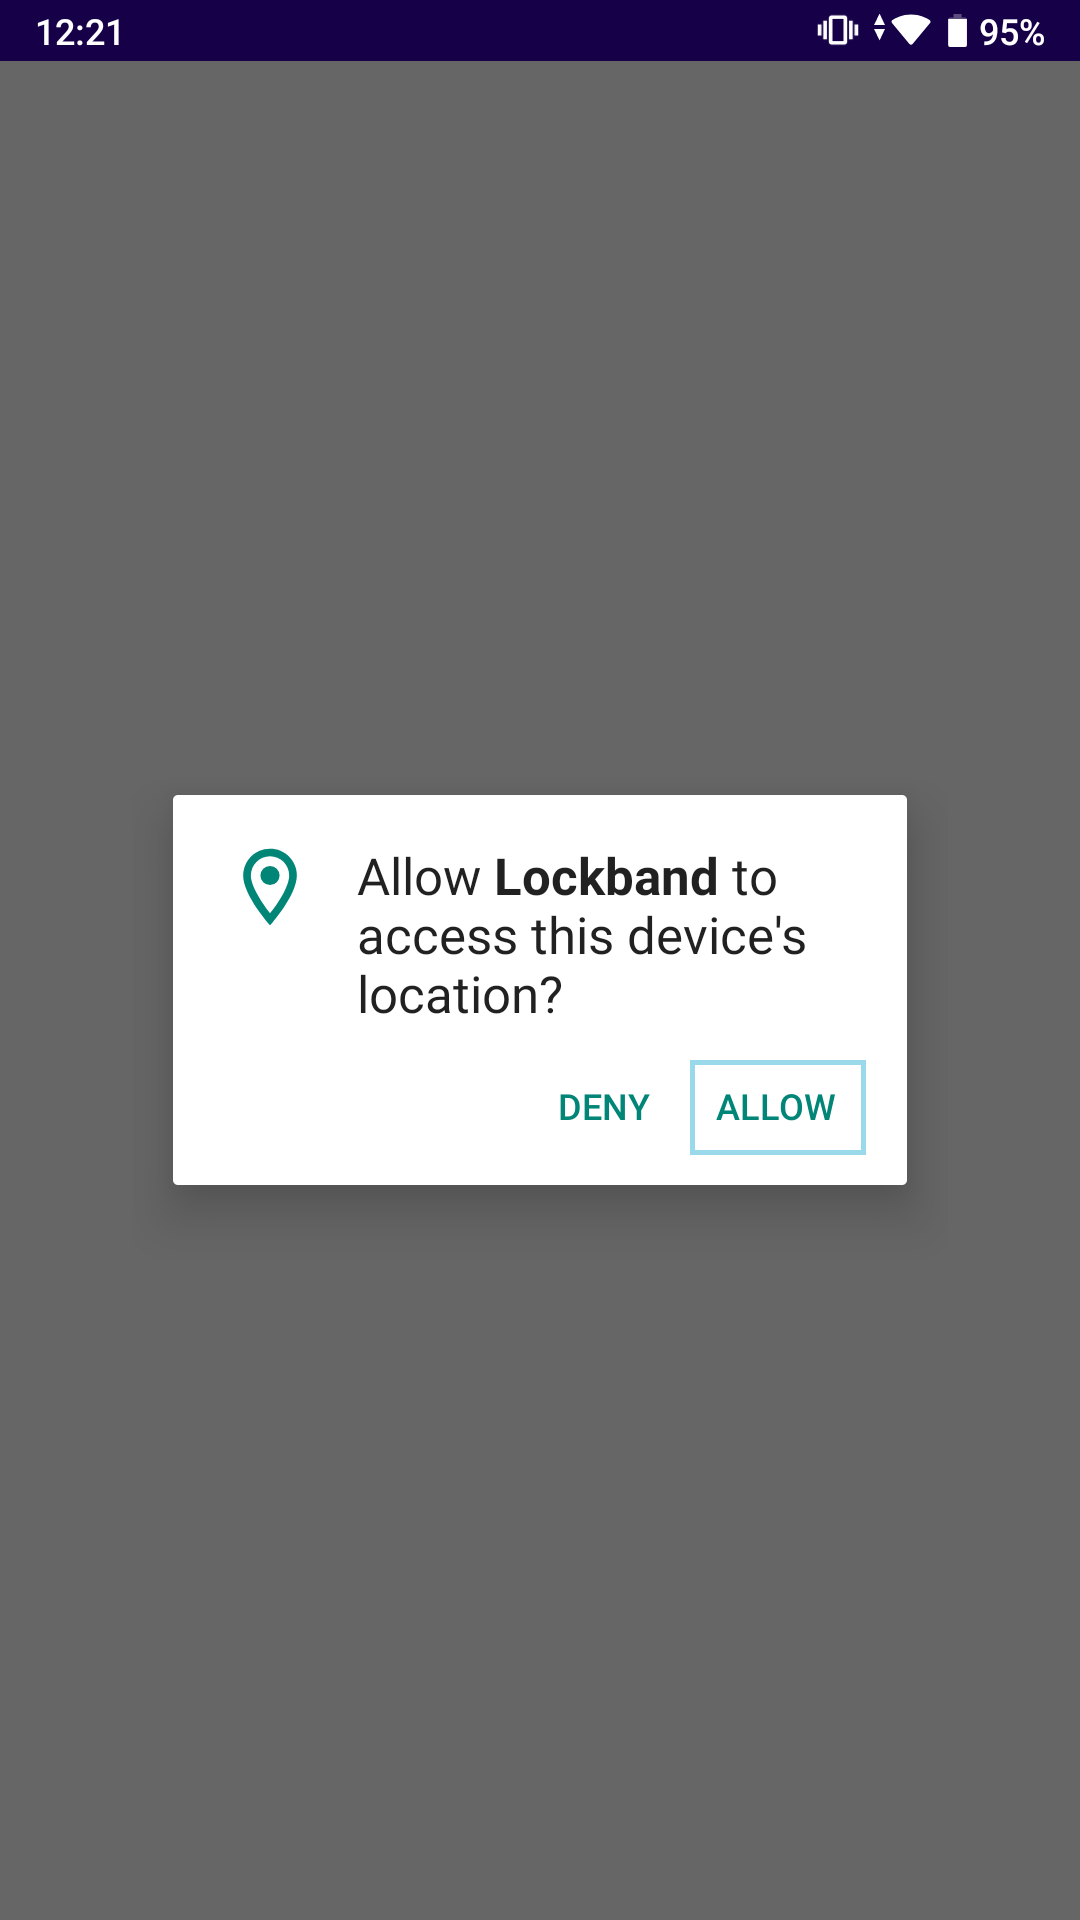
\includegraphics[width=0.27\textwidth]{app_screenshots/location_permission.png}
    \end{center}
    \caption{{\color{dgray}Udzielanie pozwoleń aplikacji.}} \label{usageStats}
\end{figure}
Kolejnym etapem konfiguracji jest ustalenie hasła, które zostanie wykorzystane do odblokowania dostępu do chronionych aplikacji. Użytkownikowi zostaje wyświetlony formularz, w którym należy wprowadzić dwa identyczne hasła, a następnie zatwierdzić je przyciskiem poniżej. Wygląd formularza można zobaczyć w poniższej grafice.
\begin{figure}[H]
    \begin{center}
        \setlength{\fboxsep}{0pt}%
        \setlength{\fboxrule}{0.27pt}%
        \fbox{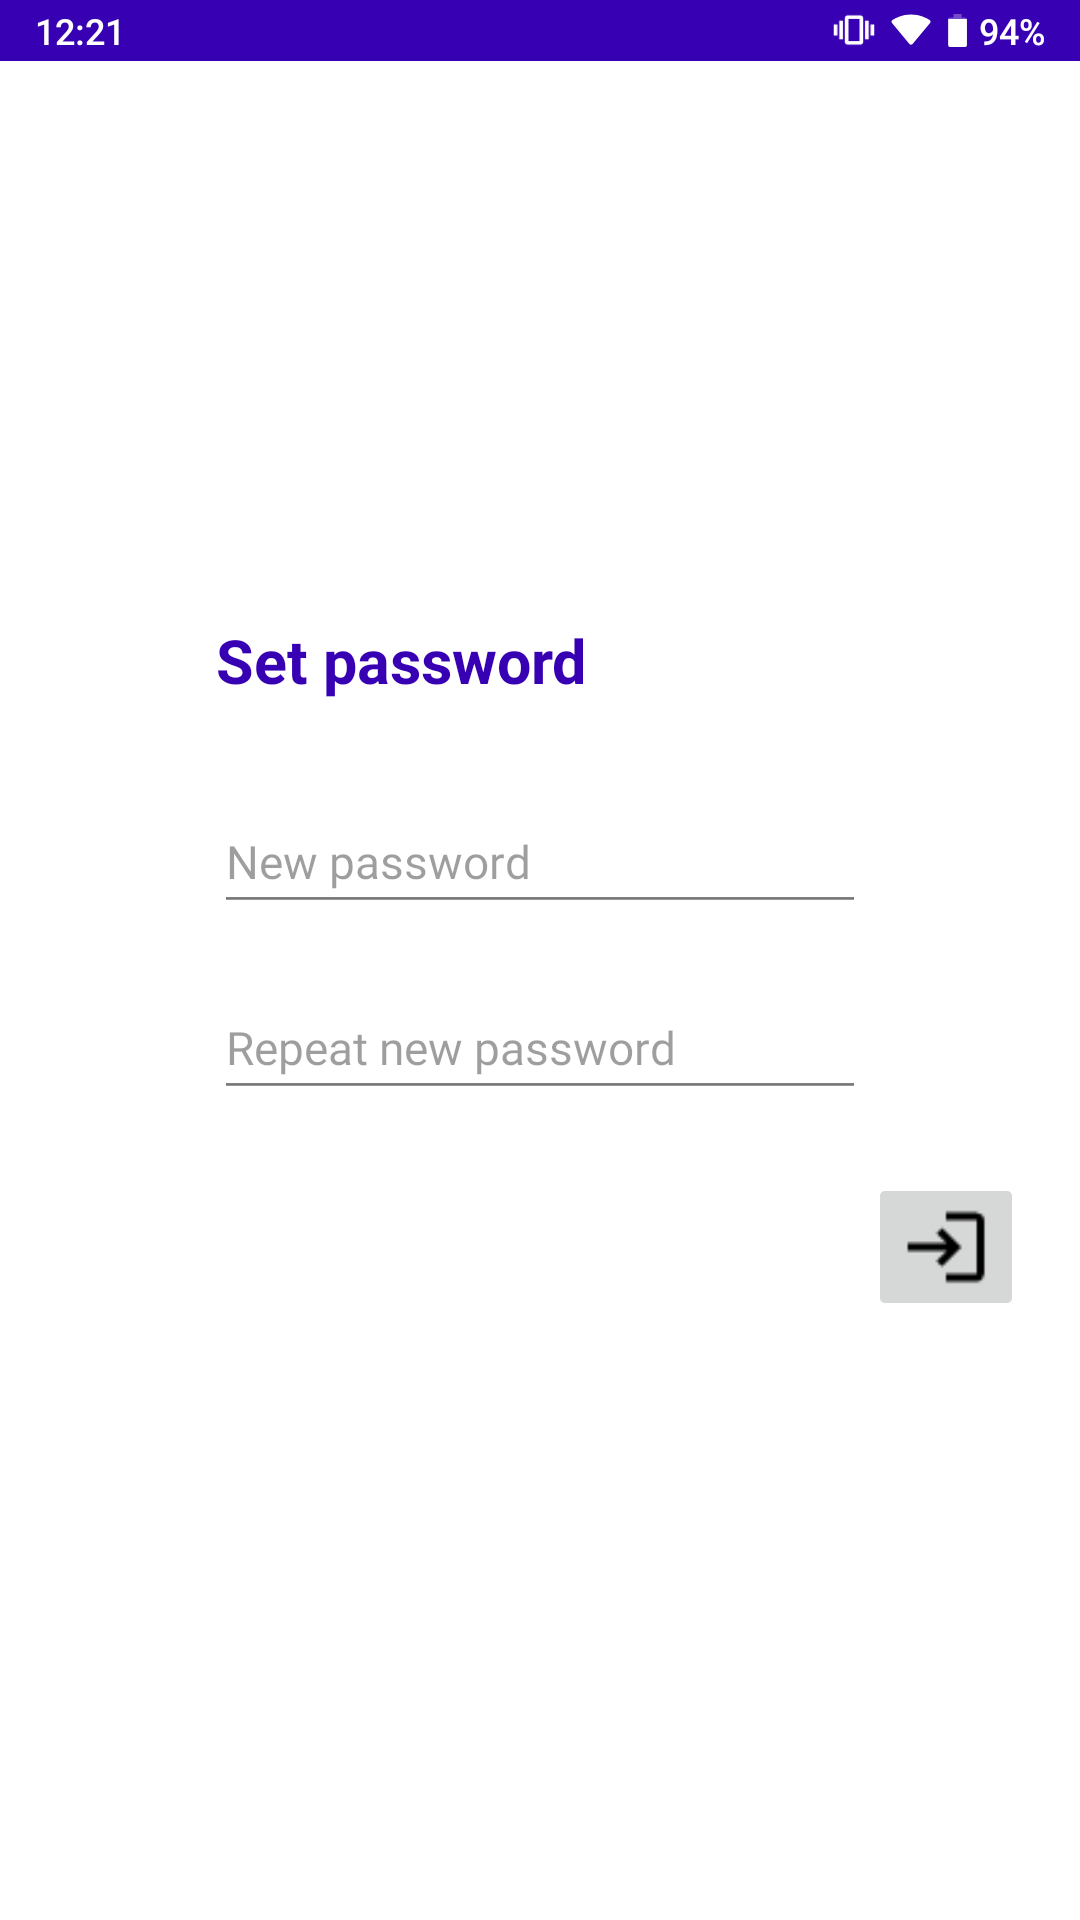
\includegraphics[width=0.3\textwidth]{app_screenshots/set_password.png}}
    \end{center}
    \caption{{\color{dgray}Formularz kreacji hasła.}} \label{setPassword}
\end{figure}
Ostatnim etapem konfiguracji jest sparowanie opaski MiBand 3 z aplikacją. W tym celu zostaje wyświetlona aktywność odpowiedzialna za skanowanie pobliskich urządzeń Bluetooth. Po naciśnięciu przycisku \textit{Scan for devices} zostaje uruchomione skanowanie z nałożonym filtrem na typ urządzenia. Jeśli za pierwszym razem opaska nie zostanie znaleziona należy powtórzyć skan. Po znalezieniu urządzenia zostaje ono wyświetlone na liście. Aby rozpocząć proces parowania należy nacisnąć nazwę danego urządzenia. Po zakończeniu parowania konfiguracja dobiega końca i użytkownik zostaje przeniesiony do głównego menu aplikacji. Inne sprawy konfiguracyjne takie, jak wybranie chronionych aplikacji czy zmiana hasła są dostępne w pozycji \textit{Settings} w menu dolnym aplikacji.
\begin{figure}[H]
    \begin{center}
        \setlength{\fboxsep}{0pt}%
        \setlength{\fboxrule}{0.27pt}%
        \fbox{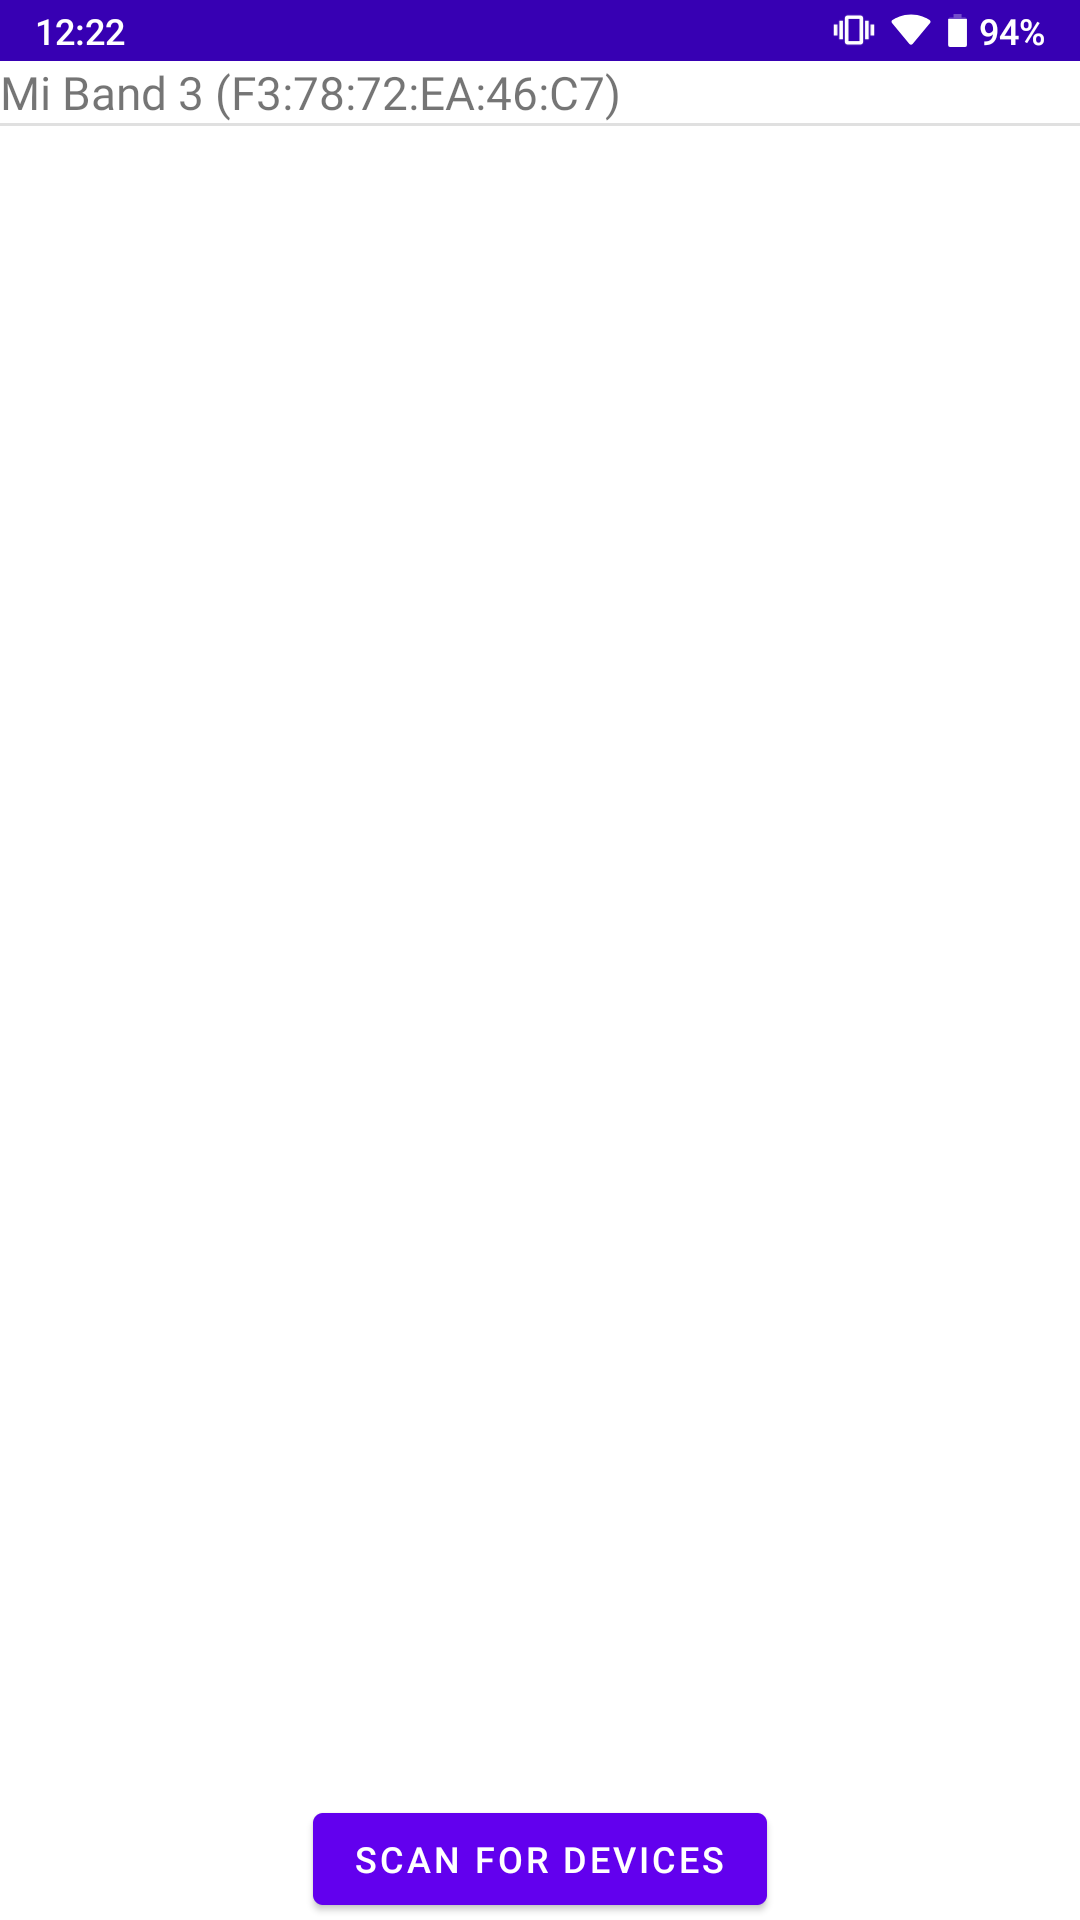
\includegraphics[width=0.27\textwidth]{app_screenshots/after_scan.png}}
    \end{center}
    \caption{{\color{dgray}Lista znalezionych w czasie skanu opasek MiBand 3.}} \label{afterScan}
\end{figure}
\begin{figure}[H]
    \begin{center}
        \setlength{\fboxsep}{0pt}%
        \setlength{\fboxrule}{0.3pt}%
        \fbox{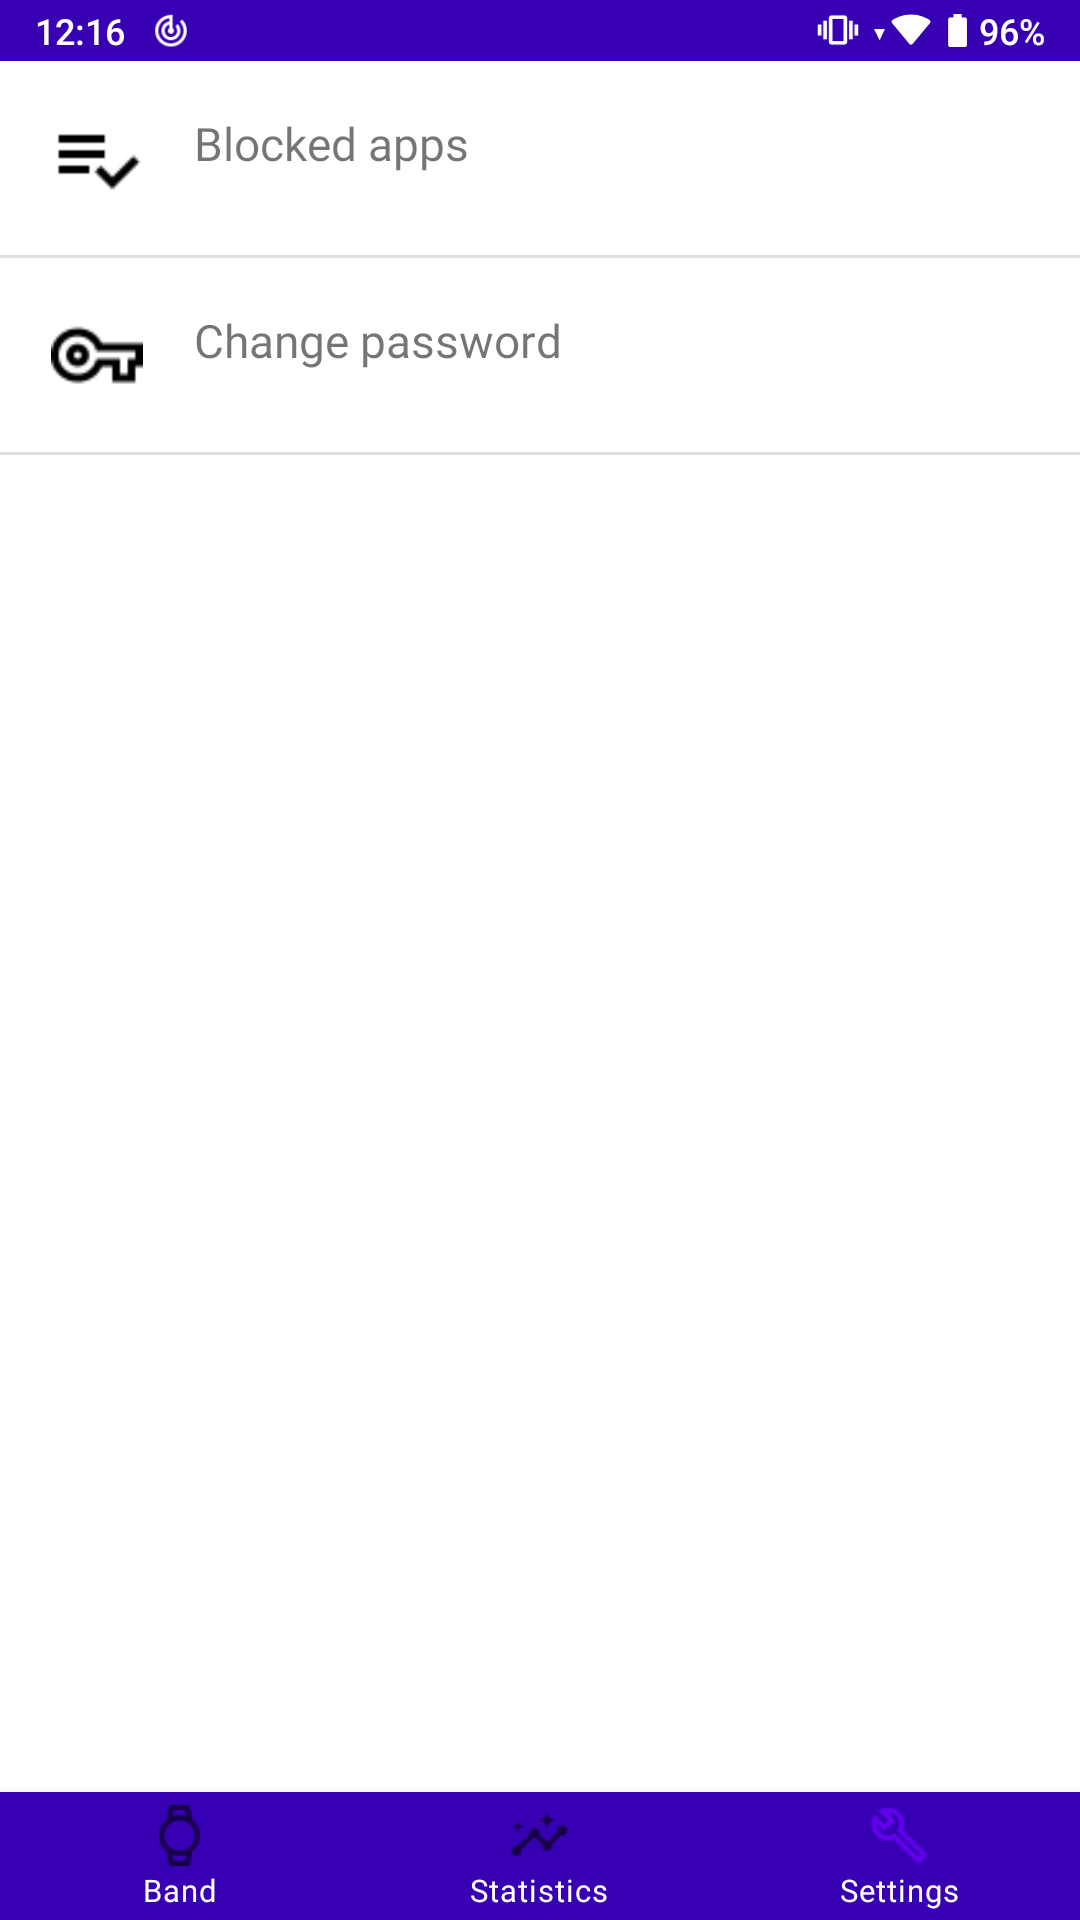
\includegraphics[width=0.27\textwidth]{app_screenshots/settings_screen.png}}
    \end{center}
    \caption{{\color{dgray}Ustawienia aplikacji.}} \label{Settings}
\end{figure}

\section{Przykłady użycia}
W tej sekcji przedstawiono jak działa aplikacja od strony użytkownika poprzez opis czynności potrzebnych do wykonania określonych zadań, np. sprawdzenie stanu opaski, zmiana blokowanych aplikacji czy sprawdzenie statystyk.
\subsection{Wybór aplikacji do zablokowania}
Aby system zapewniał należytą ochronę musi wiedzieć, co jest chronione. W tym celu należy wybrać z listy zainstalowanych aplikacji, te które będą blokowane. Do listy tej można przejść z poziomu panelu ustawień \ref{Settings}, wybierając opcję \textit{Blocked apps}. Po naciśnięciu wyświetli się lista wszystkich aplikacji znajdujących się na telefonie. Aby objąć ochroną aplikację należy wykorzystać znajdujący się przy niej przełącznik. Kiedy ma kolor niebieski, aplikacja przy próbie uruchomienia w trakcie blokady będzie przeniosić użytkownika do formularza wprowadzania hasła \ref{enterPassword}.
\begin{figure}[H]
    \begin{center}
        \setlength{\fboxsep}{0pt}%
        \setlength{\fboxrule}{0.3pt}%
        \fbox{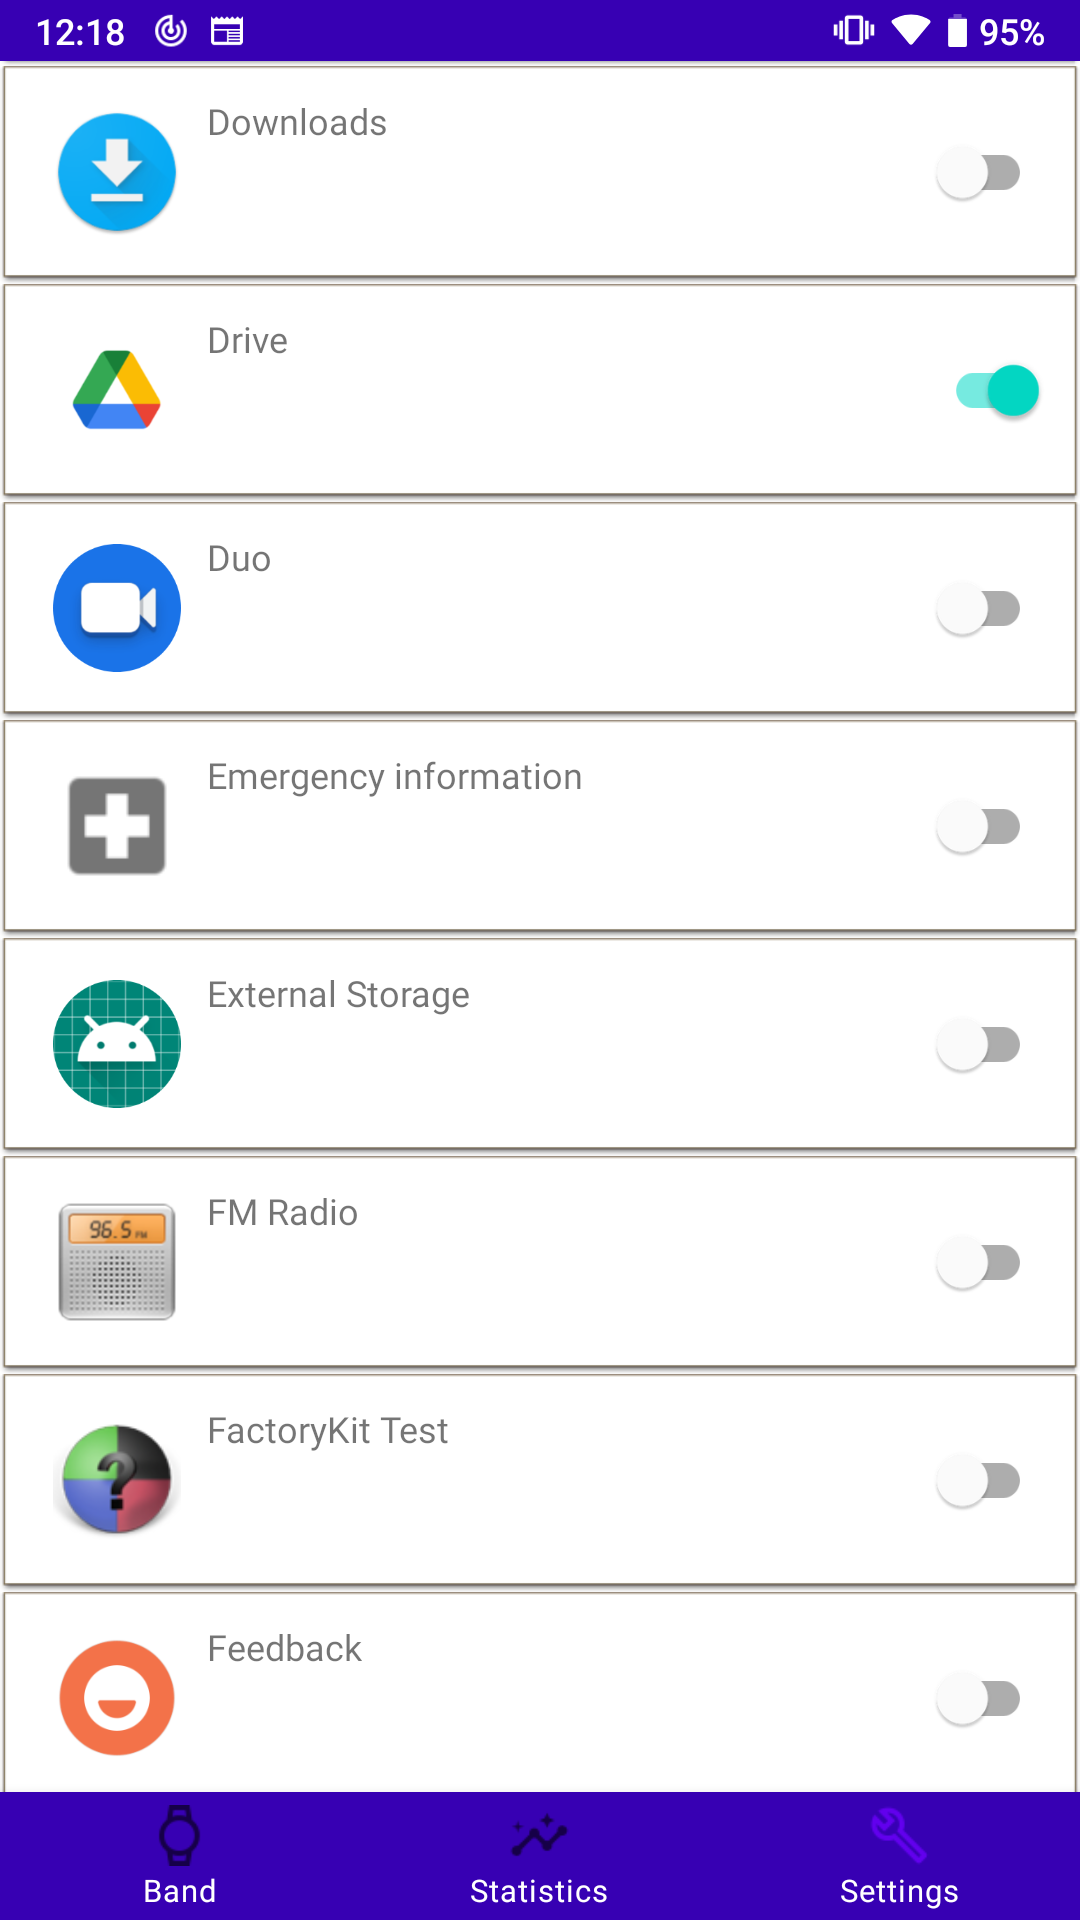
\includegraphics[width=0.27\textwidth]{app_screenshots/list_of_apps.png}}
    \end{center}
    \caption{{\color{dgray}Panel wyboru chronionych aplikacji.}} \label{appList}
\end{figure}
\subsection{Zmiana hasła użytkownika}
W przypadku, gdy użytkownik chce zmienić hasło wykorzystywane do dezaktywacji blokady, należy udać się do panelu ustawień \ref{Settings} i wybrać opcję \textit{Change password}. Po naciśnięciu pojawi się formularz zmiany hasła, gdzie należy wprowadzić stare hasło oraz dwa razy nowe hasło. Aby zapisać zmiany trzeba wcisnąć przycisk poniżej pól tekstowych.
\begin{figure}[H]
    \begin{center}
        \setlength{\fboxsep}{0pt}%
        \setlength{\fboxrule}{0.3pt}%
        \fbox{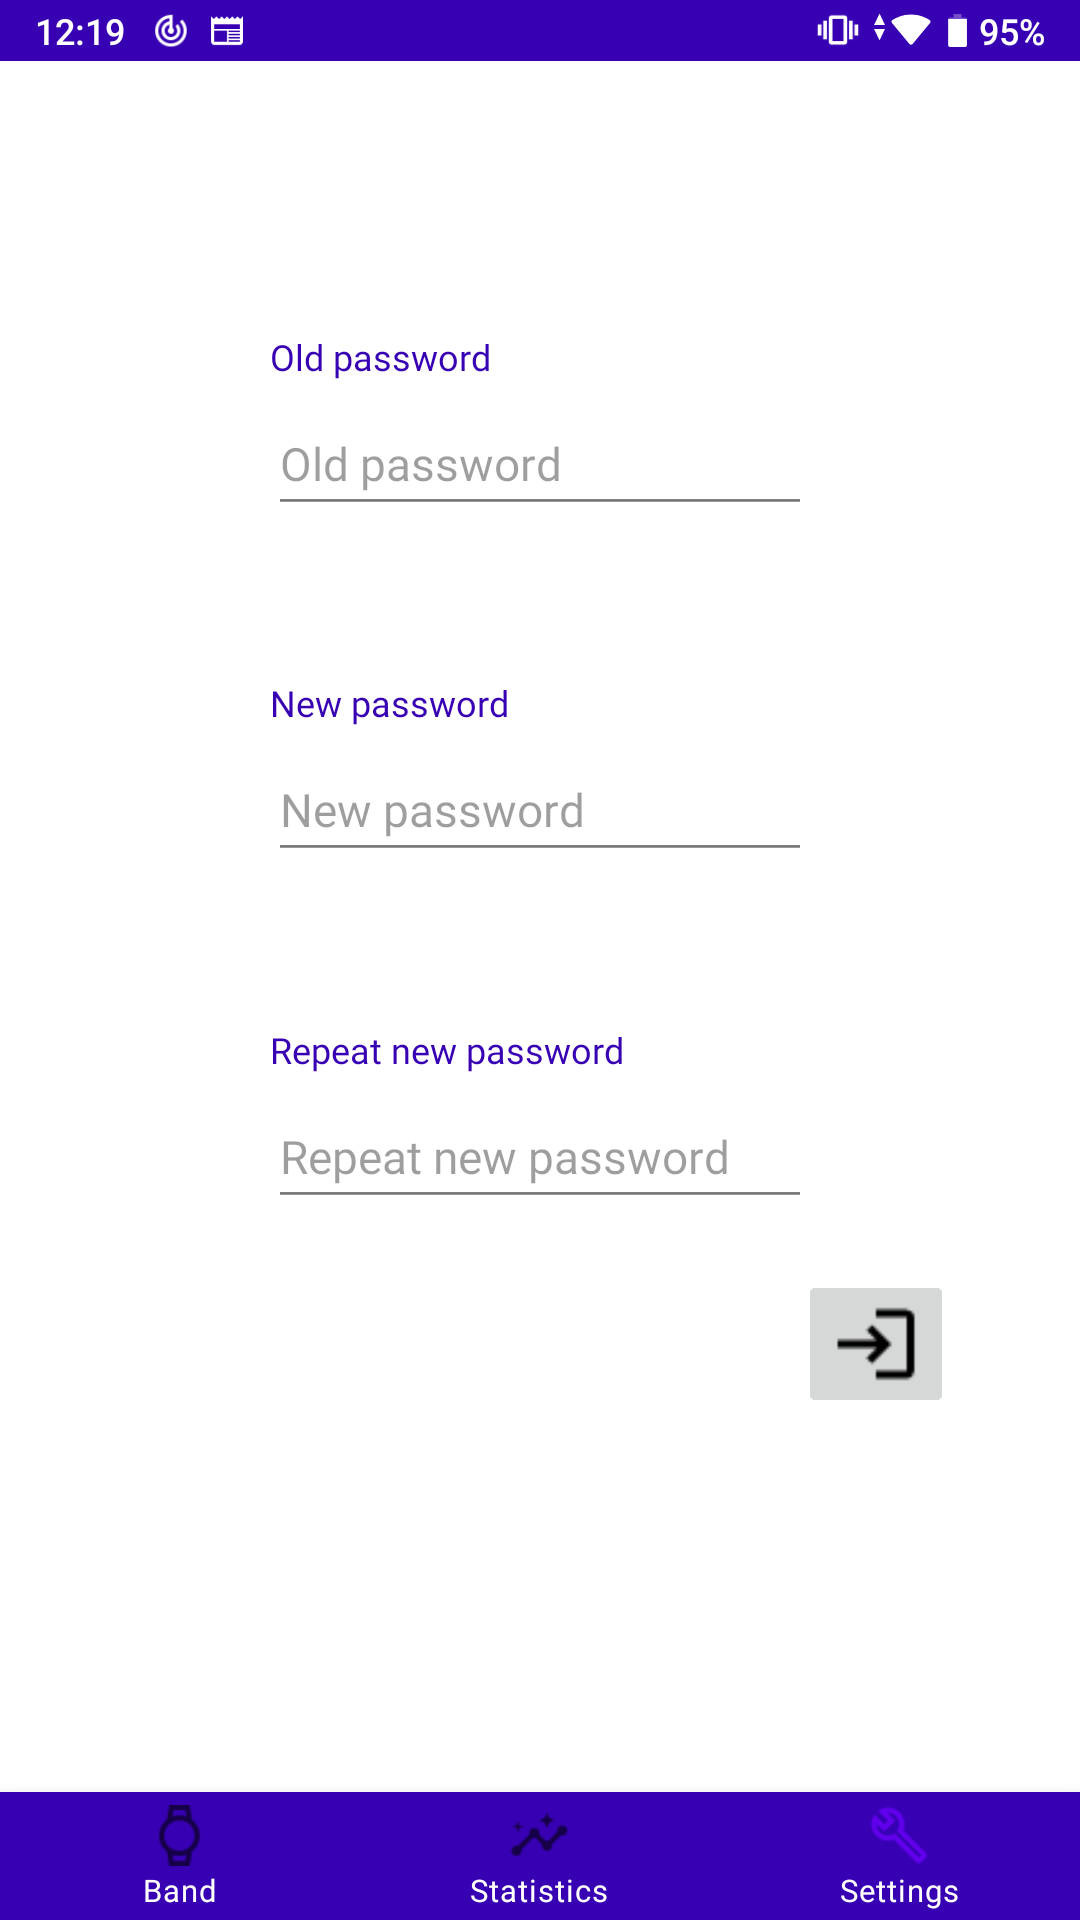
\includegraphics[width=0.27\textwidth]{app_screenshots/change_password.png}}
    \end{center}
    \caption{{\color{dgray}Panel zmiany hasła.}} \label{changePassword}
\end{figure}
\subsection{Wyświetlenie statystyk aktywności}
Aplikacja dostarcza użytkownikowi widok, w którym podane są informacje na temat zarejestrowanych danego dnia kroków oraz ostatnia wartość pomiaru pulsu. Aby zobaczyć te dane należy uruchomić aplikację oraz wybrać z dolnego menu pozycję \textit{Statistics}.
\begin{figure}[H]
    \begin{center}
        \setlength{\fboxsep}{0pt}%
        \setlength{\fboxrule}{0.3pt}%
        \fbox{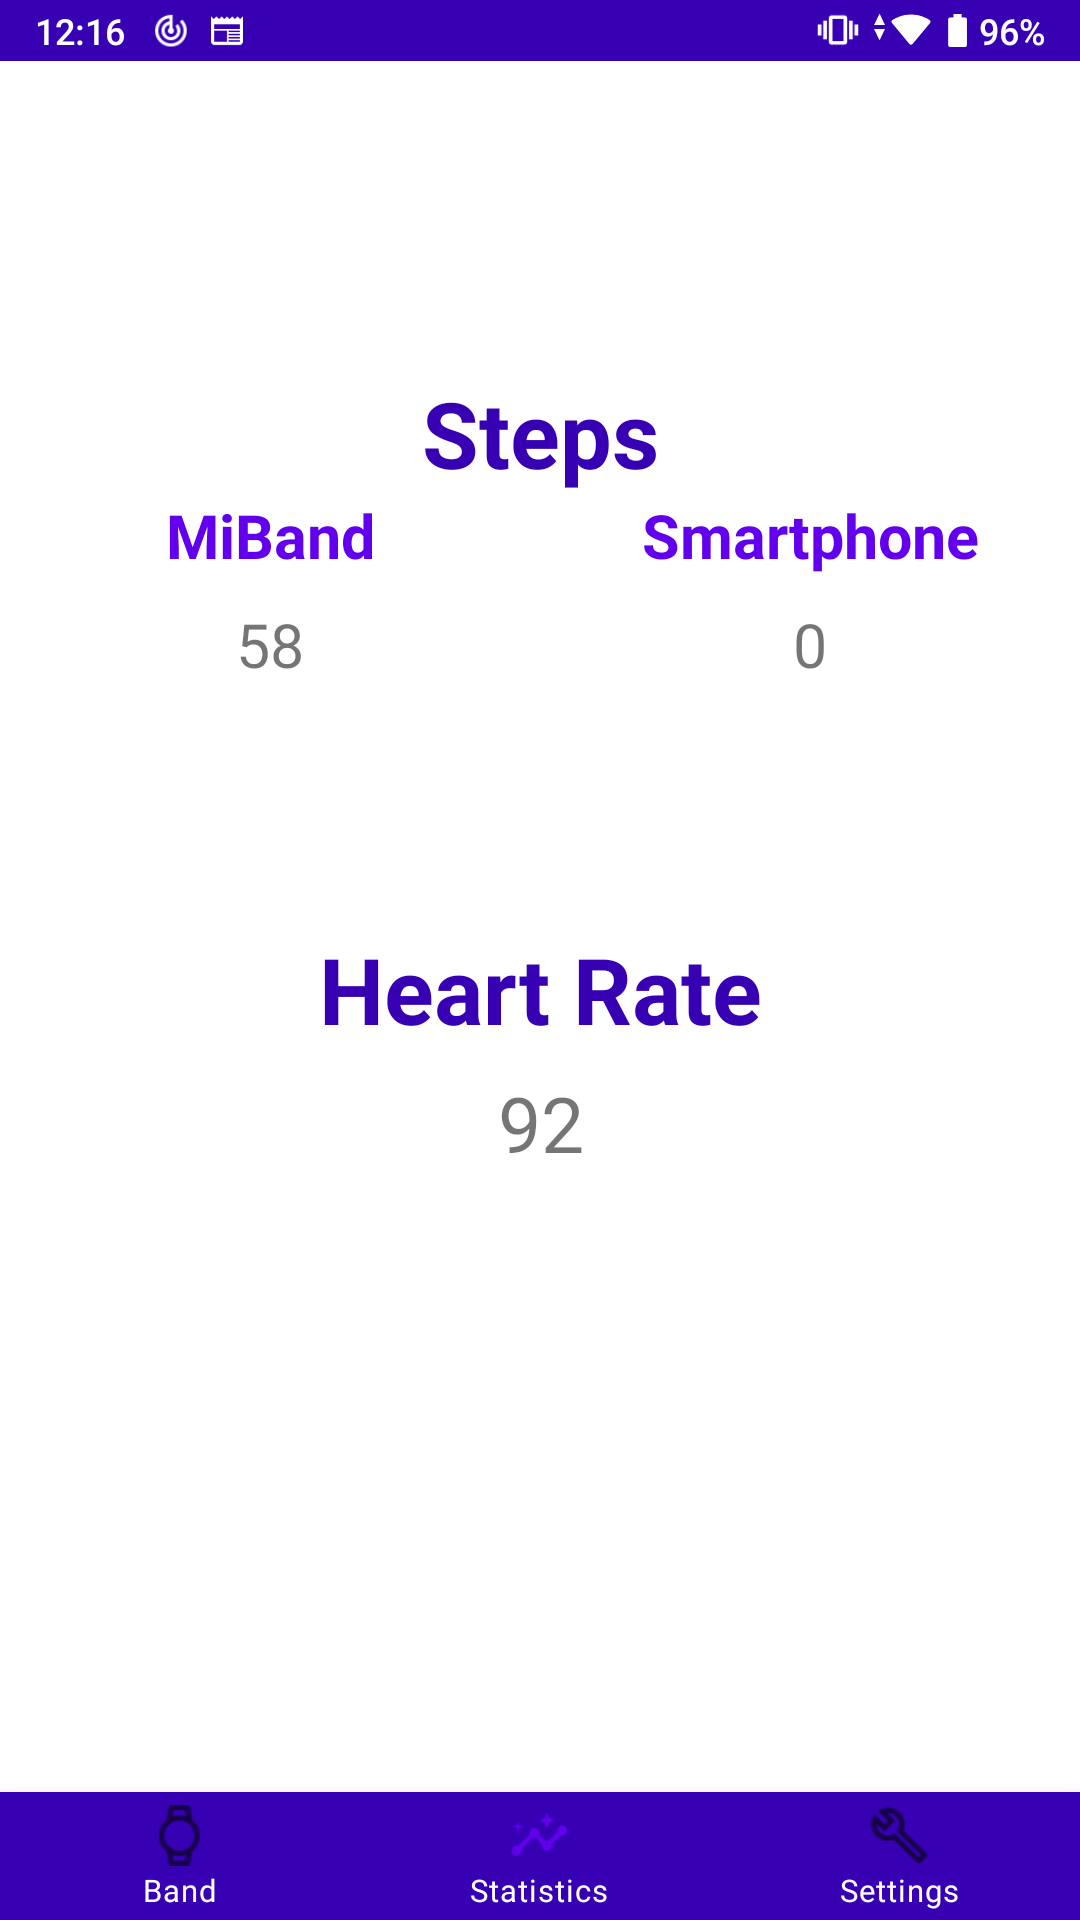
\includegraphics[width=0.27\textwidth]{app_screenshots/activity_stats.png}}
    \end{center}
    \caption{{\color{dgray}Panel informujący o ostatnich zarejestrowanych aktywnościach.}} \label{Stats}
\end{figure}
\subsection{Wyświetlenie informacji o opasce}
Aplikacja zapewnia także panel, w którym można sprawdzić podstawowe informacje o opasce oraz jej stan baterii. Aby uruchomić ten panel należy wejść do głównego widoku aplikacji i wybrać z menu dolnego pozycję \textit{Band}.
\begin{figure}[H]
    \begin{center}
        \setlength{\fboxsep}{0pt}%
        \setlength{\fboxrule}{0.3pt}%
        \fbox{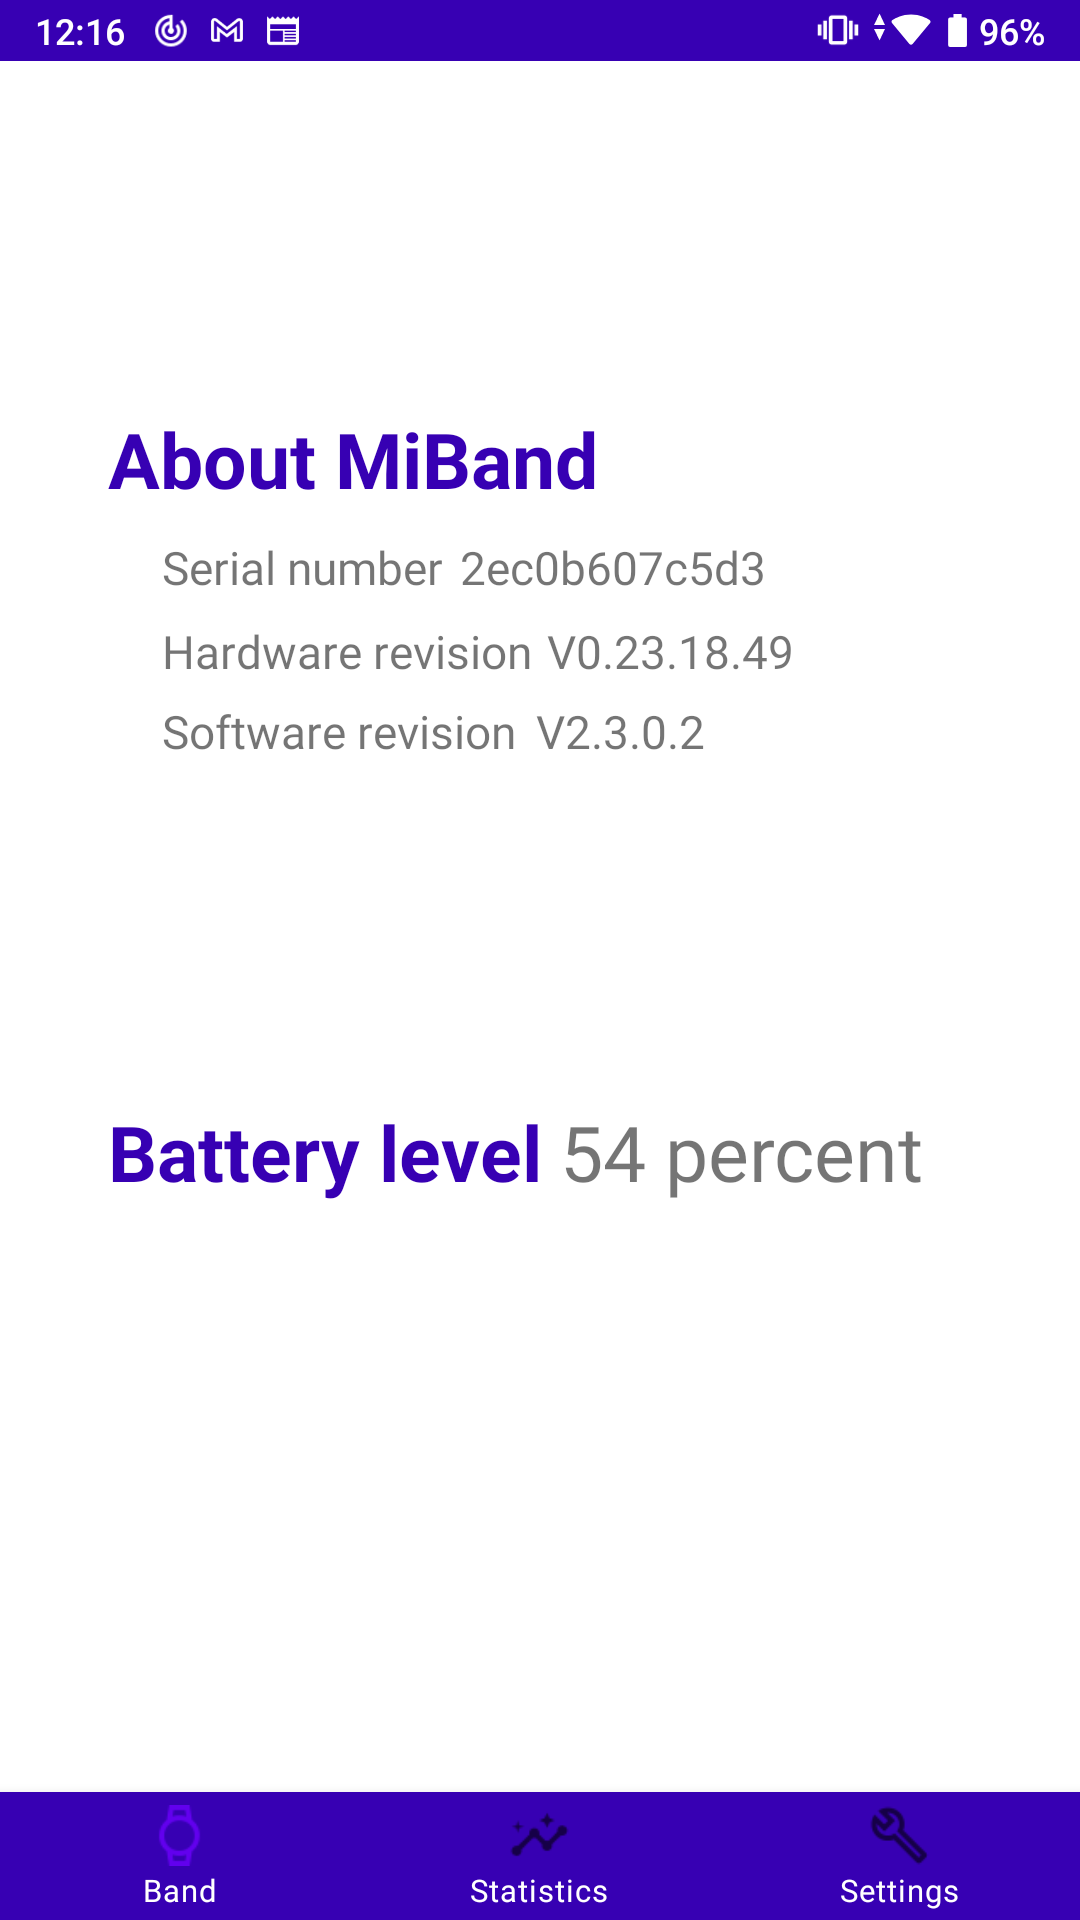
\includegraphics[width=0.27\textwidth]{app_screenshots/band_info.png}}
    \end{center}
    \caption{{\color{dgray}Panel informujący o stanie opaski.}} \label{BandInfo}
\end{figure}
\subsection{Odblokowanie systemu}
Wyłączenie aktywnej blokady odbywa się w na kilka sposobów. Użytkownik może:
\begin{itemize}
    \item nacisnąć powiadomienie o blokadzie;
    \item uruchomić aplikację;
    \item lub podjąć próbę uruchomienia jednej z chronionych aplikacji.
\end{itemize}

W każdy z tych przypadków system przekieruje użytkownika do formularza wprowadzania hasła. Po wpisaniu poprawnej wartości oraz zatwierdzeniu jej blokada zostaje zdjęta, a następnie uruchamiana jest usługa monitorująca aktywność.
\newline\newline\newline
\begin{figure}[H]
    \begin{center}
        \setlength{\fboxsep}{0pt}%
        \setlength{\fboxrule}{0.3pt}%
        \fbox{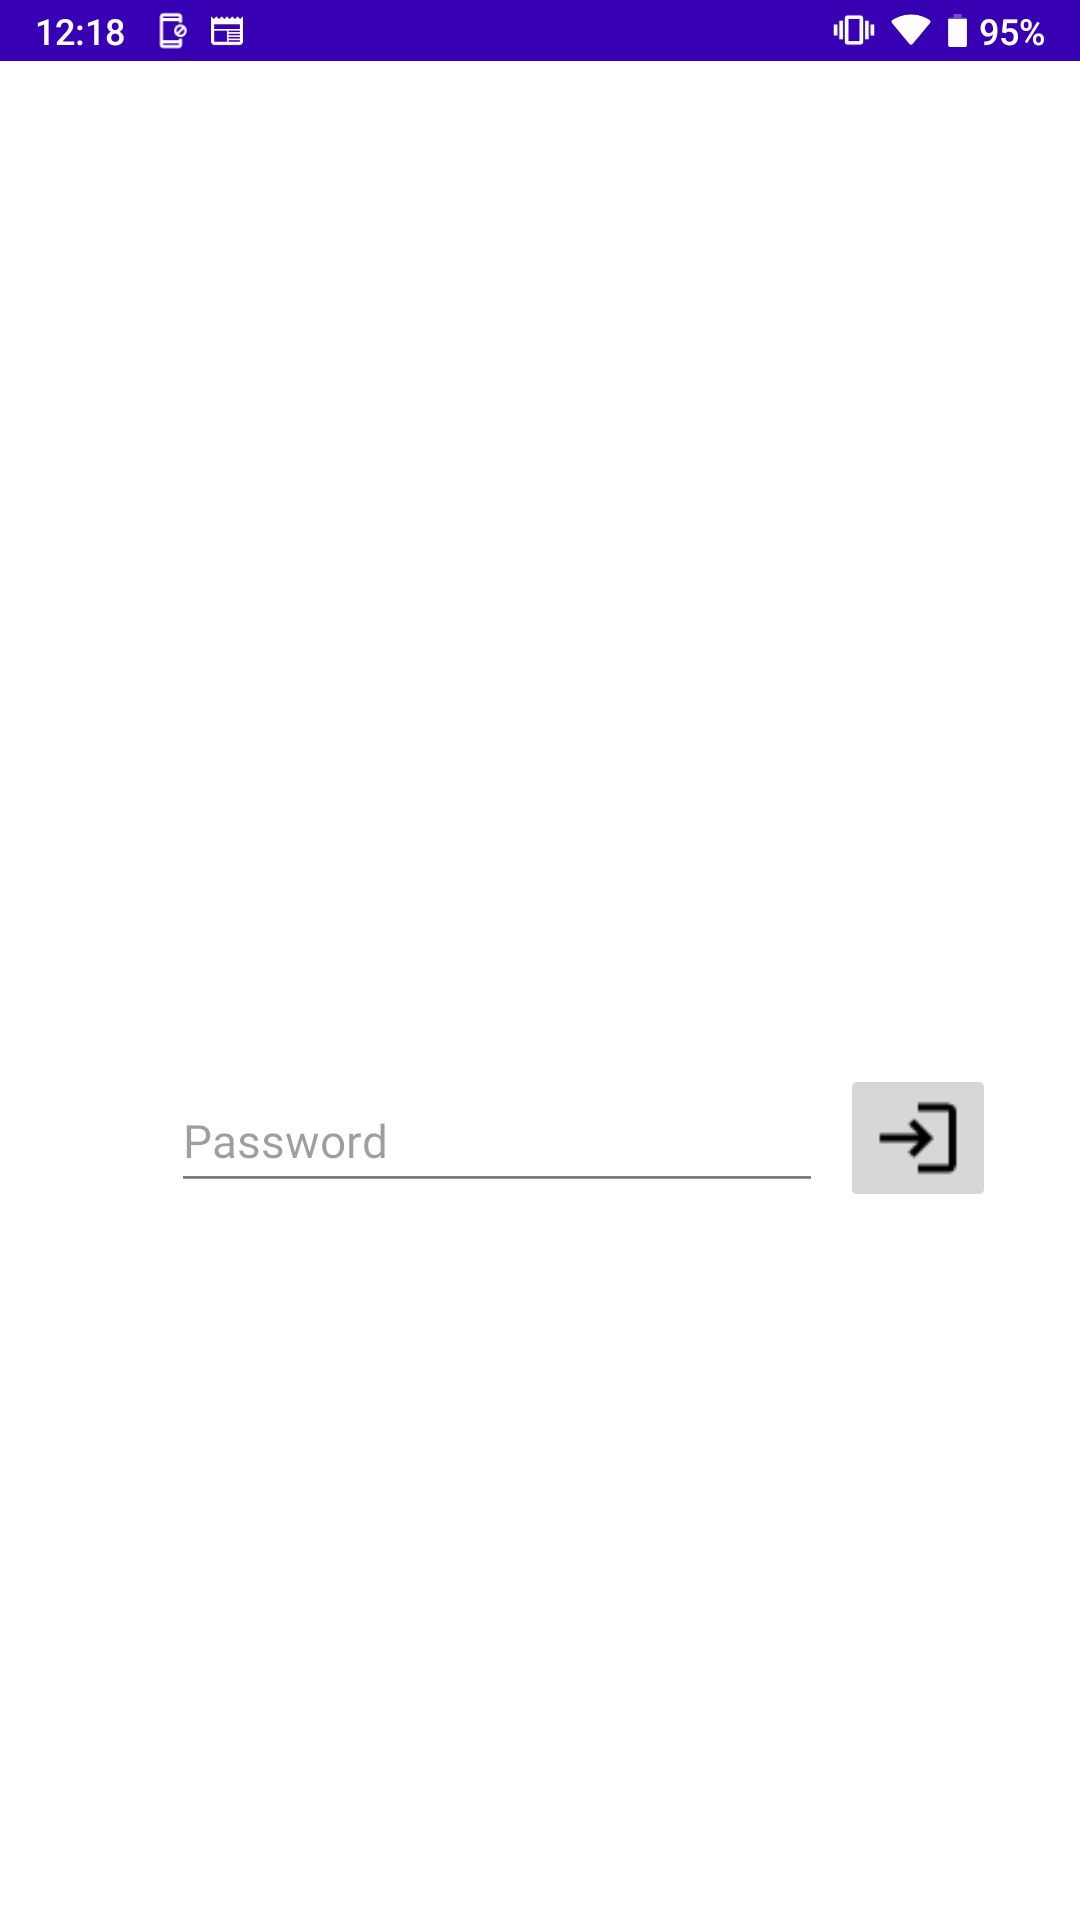
\includegraphics[width=0.27\textwidth]{app_screenshots/unblocking_activity.png}}
    \end{center}
    \caption{{\color{dgray}Formularz wprowadzania hasła.}} \label{enterPassword}
\end{figure}